\documentclass[11pt,a4paper]{article}

\usepackage[margin=1in]{geometry}
\usepackage[T1]{fontenc}
\usepackage[utf8]{inputenc}
\usepackage{lmodern}
\usepackage{setspace}
\usepackage{booktabs}
\usepackage{array}
\usepackage{graphicx}
\usepackage{xcolor}
\usepackage{hyperref}
\usepackage{enumitem}
\usepackage{amsmath}
\usepackage{float}
\usepackage{caption}

\hypersetup{
    colorlinks=true,
    linkcolor=blue!50!black,
    urlcolor=blue!50!black,
    citecolor=blue!50!black
}

\setstretch{1.15}

\title{Market Regime Detection in Indian Equities Using Hidden Markov Models}
\author{Project Report}
\date{\today}

\begin{document}

\maketitle

\section{Abstract}

This project investigates if the Hidden Markov Model (HMM) can identify market regimes in NSE-listed equities. Using daily price data for \texttt{RELIANCE.NS} from Yahoo Finance, the study constructs a feature set based on log returns, rolling volatility, and Relative Strength Index (RSI). A Gaussian HMM is fit to the feature space to infer hidden states that are interpreted as market regimes. The analysis includes both static in-sample exploration and walk-forward framework to evaluate regime detection accurately. Two trading overlays are tested: a probability-weighted strategy and a threshold-based allocation rule. Results show that the HMM is able to produce interpretable regimes, but trading performance is mixed. While some configurations improve gross Sharpe ratios, the edge deteriorates in others. The findings suggest that regime detection is useful as a risk-filtering tool, though it cannot be used as a standalone trading strategy.

\section{Introduction}

\subsection{Motivation}

A market regime identifying framework attempts to classify market behavior into a small number of recurring states. These states are not directly observed; instead, they are inferred from observable market variables. HMMs are well suited to this task because they explicitly model a state process and allow the observed feature distribution to vary across states.

\subsection{Problem Statement}

The core questions addressed in this project are:

\begin{enumerate}[label=\arabic*.]
    \item Can a Gaussian Hidden Markov Model identify economically meaningful market regimes in an Indian stock?
    \item Are the inferred regimes stable enough to be used in a walk-forward setting?
    \item Can regime probabilities support a simple allocation rule that improves risk-adjusted performance?
    \item How sensitive are results to training window choice and transaction costs?
    \item Can this work as a standalone strategy for swing-trades?
\end{enumerate}

\subsection{Prior Work}

Hamilton (1989) formalized Markov-switching models for macroeconomic time series, showing how latent regimes can explain structural changes in observed data. In financial applications, HMMs and related state-space models have been used to classify bull/bear markets, volatility states, and credit cycles.

At the same time, financial regime detection faces persistent challenges. Regimes inferred in-sample can appear cleaner than they are out-of-sample. State probabilities can be statistically sharp without necessarily translating into profitable trading signals. Frequent state switching can lead to high turnover and taxes. This project is therefore framed not only as a predictive exercise, but also as an empirical test of whether regimes by itself are actionable through strategy or not.

\section{Data \& Features}

\subsection{Sample Data Source and Sample Period}

\begin{itemize}
    \item \textbf{Asset:} \texttt{RELIANCE.NS}
    \item \textbf{Market:} NSEI
    \item \textbf{Source:} Yahoo Finance via \texttt{yfinance}
    \item \textbf{Sample Period:} January 1, 2015 to March 19, 2026
    \item \textbf{Frequency:} Daily adjusted closing prices
\end{itemize}

The project begins with a single-stock analysis to maintain interpretability and to test the workflow before generalizing to a larger cross-section.

\subsection{Feature Set}

The feature matrix is designed to capture three distinct aspects of market behavior:

\begin{enumerate}[label=\arabic*.]
    \item \textbf{Log Returns} \\
    Formula: \texttt{r\_t = 100 * log(P\_t / P\_(t-1))} \\
    Returns capture short-horizon directional movement.

    \item \textbf{Rolling Volatility} \\
    Formula: \texttt{sigma\_t = std(r\_(t-w+1), ..., r\_t)} \\
    where \texttt{w = 20} trading days. \\
    Volatility captures recent instability in returns.

    \item \textbf{Relative Strength Index (RSI)} \\
    A 14-day RSI is used to measure short-term momentum and overbought/oversold behavior.
\end{enumerate}

\subsection{Feature Configuration}

\begin{table}[H]
\centering
\begin{tabular}{lcl}
\toprule
Feature & Window & Purpose \\
\midrule
Log return & 1 day & Directional price movement \\
Rolling volatility & 20 days & Short-term risk / instability \\
RSI & 14 days & Momentum / reversal signal \\
\bottomrule
\end{tabular}
\caption{Feature construction used in the project.}
\end{table}

\subsection{Data Handling}

The feature pipeline applies the following preprocessing:

\begin{itemize}
    \item Sort index chronologically
    \item Forward-fill missing prices when necessary
    \item Drop remaining missing values
    \item Align RSI to the return index
    \item Remove rows with insufficient rolling history
\end{itemize}

This ensures that the HMM is fit on a clean, synchronized feature matrix.

\subsection{Descriptive Statistics}

Descriptive statistics for the feature matrix generated from \texttt{RELIANCE.NS} over the sample period are shown below.

\begin{table}[H]
\centering
\begin{tabular}{lrrrr}
\toprule
Variable & Mean & Std Dev & Min & Max \\
\midrule
Return & 0.0712 & 1.6990 & -14.1032 & 13.7307 \\
Volatility & 1.5529 & 0.6933 & 0.5570 & 7.7406 \\
RSI & 52.9987 & 16.7960 & 7.7226 & 97.5634 \\
\bottomrule
\end{tabular}
\caption{Descriptive statistics of the feature matrix.}
\end{table}

The same values can be reproduced from the project pipeline using the following code:

\begin{verbatim}
from src.utils import load_config
from src.data_fetcher import fetch_data
from src.features import build_feature_matrix

config = load_config('config/config.yaml')
prices = fetch_data(config['ticker'], config['start_date'], config['end_date'])
features = build_feature_matrix(prices, config)
print(features.describe().T)
\end{verbatim}

\subsection{Figures}

The following figures are already generated by the walk-forward script and can be embedded directly in the report.

\begin{figure}[H]
    \centering
    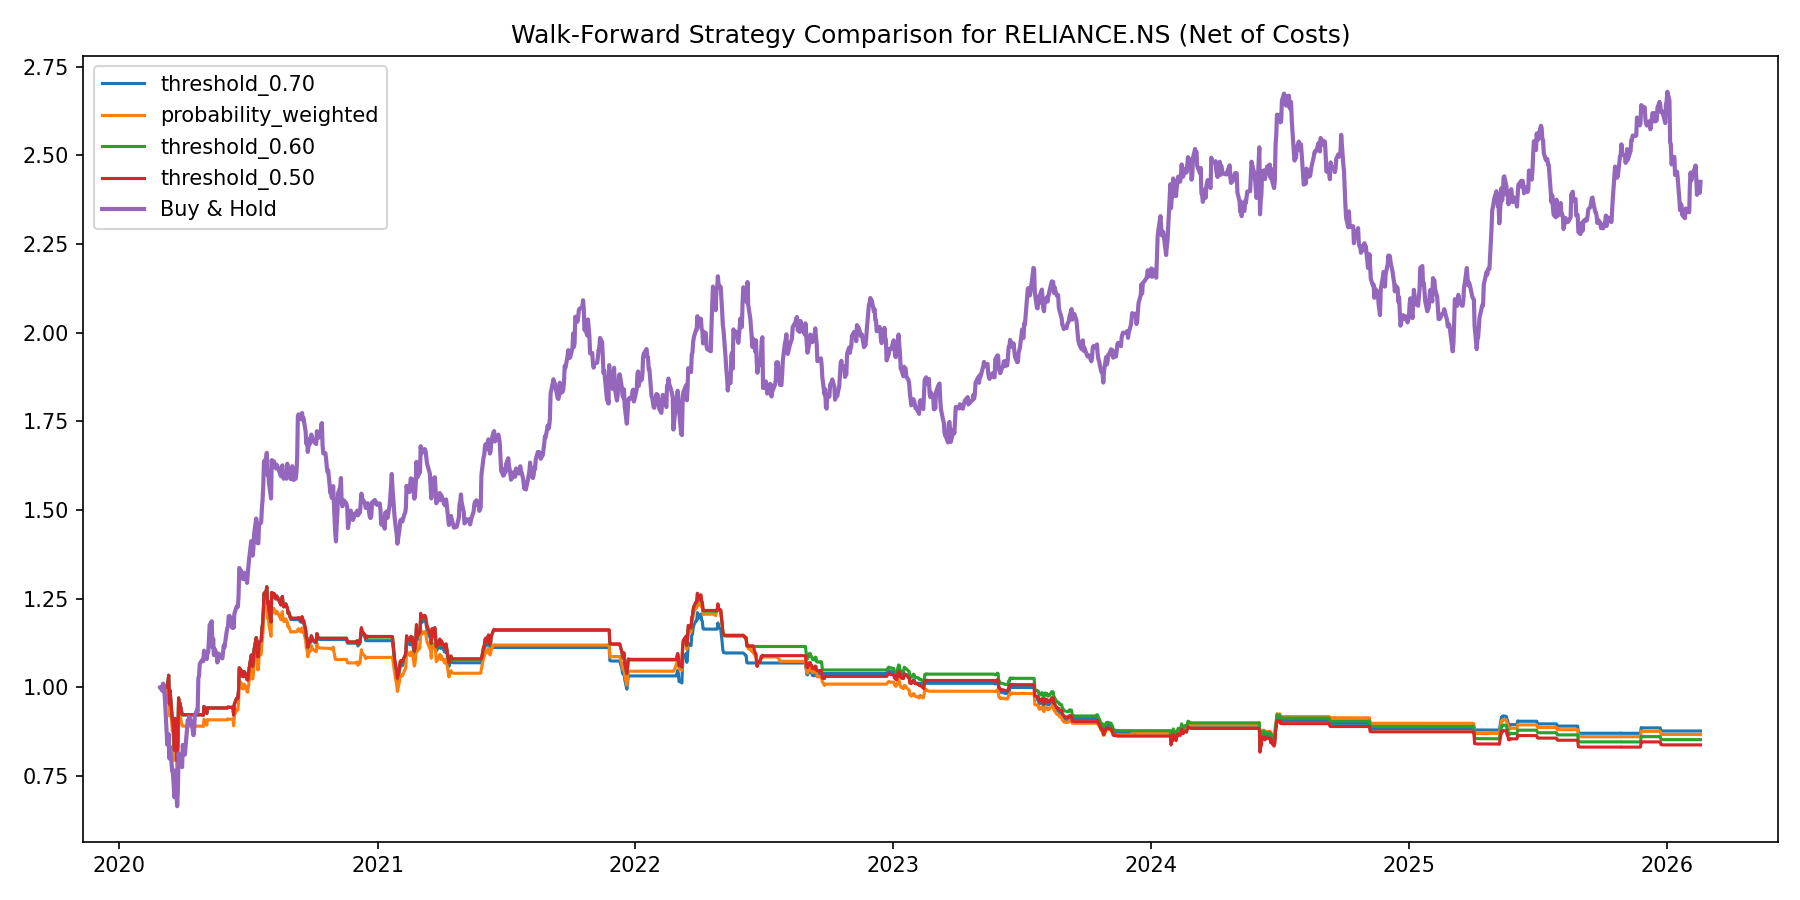
\includegraphics[width=0.9\textwidth]{outputs/figures/walk_forward_equity_RELIANCE_NS_1250_20.png}
    \caption{Equity curve generated by the walk-forward script.}
\end{figure}

\begin{figure}[H]
    \centering
    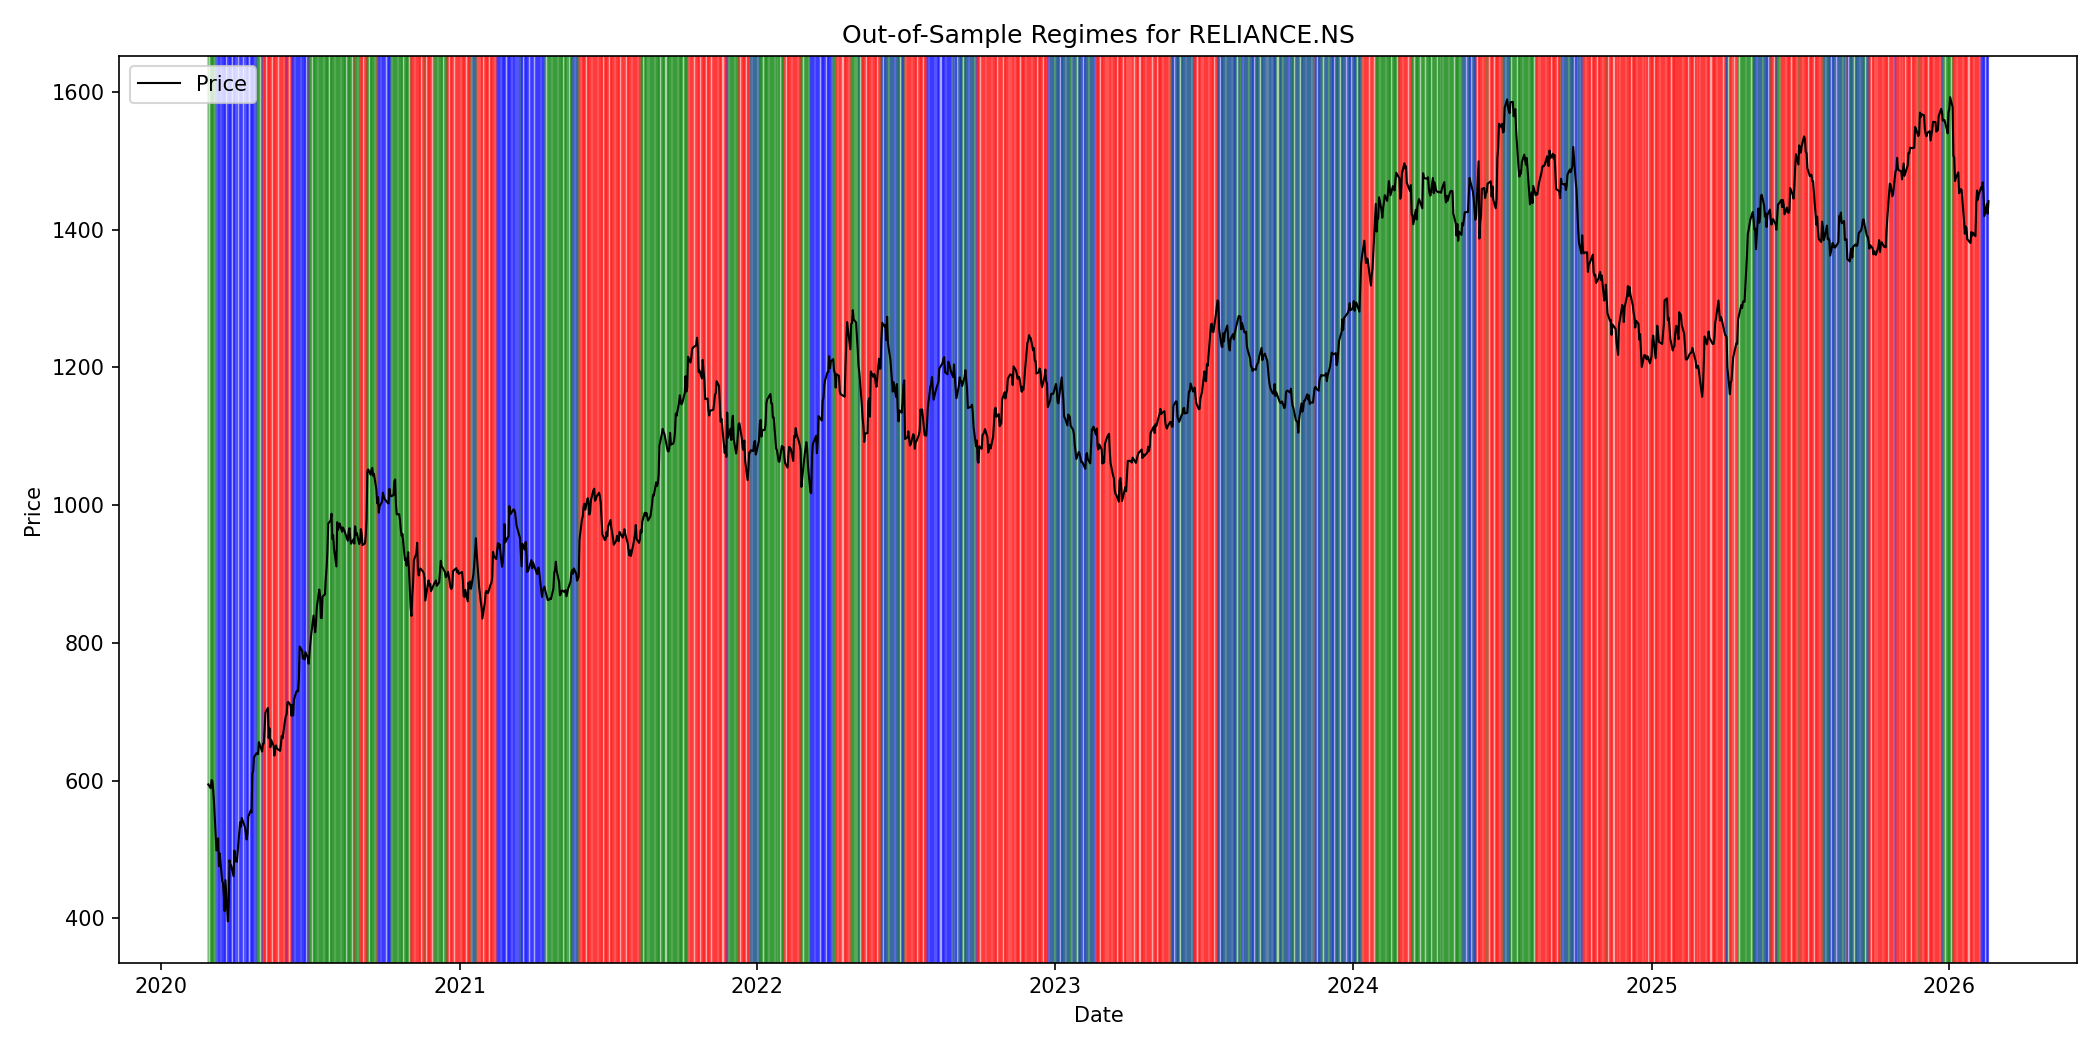
\includegraphics[width=0.9\textwidth]{outputs/figures/walk_forward_regimes_RELIANCE_NS_1250_20.png}
    \caption{Out-of-sample regime plot generated by the walk-forward script.}
\end{figure}

\begin{figure}[H]
    \centering
    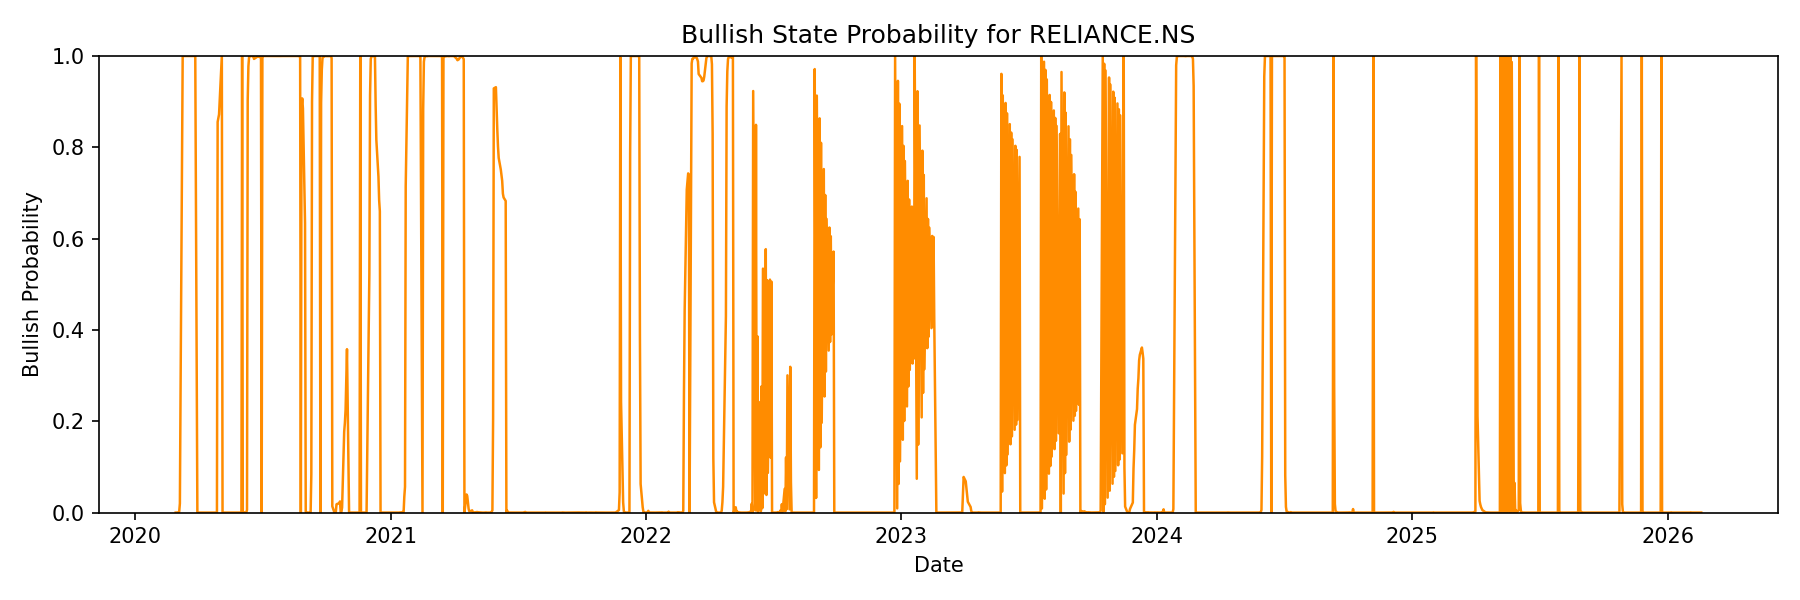
\includegraphics[width=0.9\textwidth]{outputs/figures/walk_forward_probs_RELIANCE_NS_1250_20.png}
    \caption{Posterior probability plot generated by the walk-forward script.}
\end{figure}

\end{document}
